% Copyright (c) 2022 by Lars Spreng
\newcommand{\mycopyright}{%
  \small
  Copyright (c) 2022 by Lars Spreng.
  This work is licensed under the Creative Commons Attribution 4.0 International License. 
  To view a copy of this license, visit \url{http://creativecommons.org/licenses/by/4.0/} or send a letter to Creative Commons, PO Box 1866, Mountain View, CA 94042, USA.
}
% This work is licensed under the Creative Commons Attribution 4.0 International License. 
% To view a copy of this license, visit http://creativecommons.org/licenses/by/4.0/ or send a letter to Creative Commons, PO Box 1866, Mountain View, CA 94042, USA.

%~~~~~~~~~~~~~~~~~~~~~~~~~~~~~~~~~~~~~~~~~~~~~~~~~~~~~~~~~~~~~~~~~~~~~~~~~~~~~~
% You can add your packages and commands to the loadslides.tex file. 
% The files in the folder "styles" can be modified to change the layout and design of your slides.
% I have included examples on how to use the template below. 
% Some of it these examples are taken from the Metropolis template.
%~~~~~~~~~~~~~~~~~~~~~~~~~~~~~~~~~~~~~~~~~~~~~~~~~~~~~~~~~~~~~~~~~~~~~~~~~~~~~~


\documentclass[
11pt,notheorems,hyperref={pdfauthor=whatever}
]{beamer}


% Copyright (c) 2022 by Lars Spreng
% This work is licensed under the Creative Commons Attribution 4.0 International License. 
% To view a copy of this license, visit http://creativecommons.org/licenses/by/4.0/ or send a letter to Creative Commons, PO Box 1866, Mountain View, CA 94042, USA.

%~~~~~~~~~~~~~~~~~~~~~~~~~~~~~~~~~~~~~~~~~~~~~~~~~~~~~~~~~~~~~~~~~~~~~~~~~~~~~~
% Add your packages and commands to this file
%~~~~~~~~~~~~~~~~~~~~~~~~~~~~~~~~~~~~~~~~~~~~~~~~~~~~~~~~~~~~~~~~~~~~~~~~~~~~~~



%~~~~~~~~~~~~~~~~~~~~~~~~~~~~~~~~~~~~~~~~~~~~~~~~~~~~~~~~~~~~~~~~~~~~~~~~~~~~~~
\RequirePackage{palatino}
\RequirePackage[utf8]{inputenc}
\RequirePackage[T1]{fontenc}
\RequirePackage{}
\usepackage{intcalc}
\usefonttheme{serif}

\usepackage{styles/elegantmacros}
\usefolder{styles}
\usetheme[style=blue]{elegant}



\newcommand{\makepart}[1]{ % For convenience
\part{#1} \frame{\partpage}
}

%~~~~~~~~~~~~~~~~~~~~~~~~~~~~~~~~~~~~~~~~~~~~~~~~~~~~~~~~~~~~~~~~~~~~~~~~~~~~~~

%~~~~~~~~~~~~~~~~~~~~~~~~~~~~~~~~~~~~~~~~~~~~~~~~~~~~~~~~~~~~~~~~~~~~~~~~~~~~~~
% Figures
\RequirePackage{booktabs}
\RequirePackage{colortbl}
\RequirePackage{ragged2e}
\RequirePackage{schemabloc}
%\RequirePackage{natbib}
\RequirePackage{caption}
\RequirePackage{subcaption}
\RequirePackage{tabularx}
\RequirePackage{colortbl}
\RequirePackage{array}
\RequirePackage{multirow}
\usepackage[
  style=authoryear, 
]{biblatex}
\addbibresource{references.bib}
\newcolumntype{Y}{>{\centering\arraybackslash}X}

%~~~~~~~~~~~~~~~~~~~~~~~~~~~~~~~~~~~~~~~~~~~~~~~~~~~~~~~~~~~~~~~~~~~~~~~~~~~~~~

%~~~~~~~~~~~~~~~~~~~~~~~~~~~~~~~~~~~~~~~~~~~~~~~~~~~~~~~~~~~~~~~~~~~~~~~~~~~~~~
% Figures
\RequirePackage{wrapfig}
\usepackage{pgfplots}
\pgfplotsset{compat=1.18}
\RequirePackage{graphicx}
\RequirePackage{adjustbox}
\RequirePackage{environ}
%\pgfplotsset{compat=1.18}


\makeatletter
\RequirePackage{tikz}
\usepgfplotslibrary{fillbetween}
\usetikzlibrary{patterns, shapes.geometric}
    
\newsavebox{\measure@tikzpicture}
\NewEnviron{scaletikzpicturetowidth}[1]{%
  \def\tikz@width{#1}%
  \def\tikzscale{1}\begin{lrbox}{\measure@tikzpicture}%
  \BODY
  \end{lrbox}%
  \pgfmathparse{#1/\wd\measure@tikzpicture}%
  \edef\tikzscale{\pgfmathresult}%
  \BODY
}
\usetikzlibrary{ducks}
\makeatother
%~~~~~~~~~~~~~~~~~~~~~~~~~~~~~~~~~~~~~~~~~~~~~~~~~~~~~~~~~~~~~~~~~~~~~~~~~~~~~~

%~~~~~~~~~~~~~~~~~~~~~~~~~~~~~~~~~~~~~~~~~~~~~~~~~~~~~~~~~~~~~~~~~~~~~~~~~~~~~~
% Colors

\definecolor{sangue}{HTML}{780000}
\definecolor{sanguechiaro}{HTML}{C1121F}
\definecolor{muro}{HTML}{FDF0D5}
\definecolor{sera}{HTML}{003049}
\definecolor{macchina}{HTML}{669BBC}

%~~~~~~~~~~~~~~~~~~~~~~~~~~~~~~~~~~~~~~~~~~~~~~~~~~~~~~~~~~~~~~~~~~~~~~~~~~~~~~
%My fun

\newcommand{\myemph}[1]{\textcolor{sera}{#1}}

 %~~~~~~~~~~~~~~~~~~~~~~~~~~~~~~~~~~~~~~~~~~~~~~~~~~~~~~~~~~~~~~~~~~~~~~~~~~~~~~

%~~~~~~~~~~~~~~~~~~~~~~~~~~~~~~~~~~~~~~~~~~~~~~~~~~~~~~~~~~~~~~~~~~~~~~~~~~~~~~
% Maths 
\RequirePackage{textcomp}
\RequirePackage{amsmath} 
\RequirePackage{amsthm}
\RequirePackage{mathtools}
\usepackage{amsfonts}
\usepackage{amssymb}
\usepackage{eurosym}
\usepackage{float}
\usepackage{xfrac}
\usepackage{mathrsfs} 

%\RequirePackage{bbm}
%\RequirePackage{algorithm}
%\RequirePackage[osf,sc]{mathpazo}
%\RequirePackage{pifont}
%\newcommand{\xmark}{\ding{55}}%
%\numberwithin{equation}{section}
\DeclareMathOperator*{\argmax}{arg\,max}
\DeclareMathOperator*{\argmin}{arg\,min}

%define theorems
% \newtheorem{assumption}{Assumption}
% \newtheorem{theorem}{Theorem}
\newtheorem{prop}{Proposition}
\newtheorem{observation}{Observation}

% Define mathematical symbols
\newcommand{\nc}{\newcommand}
\nc{\sS}{ \mathscr{S}}
\nc{\sC}{ \mathscr{C}}
\nc{\cH}{{\mathcal H}}
\nc{\cR}{{\mathcal R}}
\nc{\cA}{{\mathcal A}}
\nc{\cG}{{\mathcal G}}
\nc{\cC}{{\mathcal C}}
\nc{\cD}{{\mathcal D}}
\nc{\cO}{{\mathcal O}}
\nc{\cI}{{\mathcal I}}
\nc{\cB}{{\mathcal B}}
\nc{\cY}{{\mathcal Y}}
\nc{\cK}{{\mathcal K}} 
\nc{\cX}{{\mathcal X}}
\nc{\cS}{{\mathcal S}}
\nc{\cE}{{\mathcal E}}
\nc{\cF}{{\mathcal F}}
\nc{\cZ}{{\mathcal Z}}
\nc{\cQ}{{\mathcal Q}}
\nc{\cP}{{\mathcal P}}
\nc{\cL}{{\mathcal L}}
\nc{\cM}{{\mathcal M}}
\nc{\cN}{{\mathcal N}}
\nc{\cT}{{\mathcal T}}
\nc{\cW}{{\mathcal W}}
\nc{\cU}{{\mathcal U}}
\nc{\cJ}{{\mathcal J}}
\nc{\cV}{{\mathcal V}}
\nc{\bH}{{\mathbb H}}
\nc{\bA}{{\mathbb A}}
\nc{\bG}{{\mathbb G}}
\nc{\bC}{{\mathbb C}}
\nc{\bO}{{\mathbb O}}
\nc{\bI}{{\mathbb I}}
\nc{\bB}{{\mathbb B}}
\nc{\bY}{{\mathbb Y}}
\nc{\bK}{{\mathbb K}} 
\nc{\bX}{{\mathbb X}}
\nc{\bS}{{\mathbb S}}
\nc{\bE}{{\mathbb E}}
\nc{\bF}{{\mathbb F}}
\nc{\bZ}{{\mathbb Z}}
\nc{\bQ}{{\mathbb Q}}
\nc{\bN}{{\mathbb N}}
\nc{\bP}{{\mathbb P}}
\nc{\bL}{{\mathbb L}}
\nc{\bM}{{\mathbb M}}
\nc{\bT}{{\mathbb T}}
\nc{\bW}{{\mathbb W}}
\nc{\bU}{{\mathbb U}}
\nc{\bD}{{\mathbb D}}
\nc{\bJ}{{\mathbb J}}
\nc{\bV}{{\mathbb V}}
\nc{\bR}{{\mathbb R}}

% & \frac{1}{J} \sum_{s \in \cJ} \sum_{t \in \cT} \Bigg(\sum_{i \in \netN}
% \left( c_i^\aHtE \HtEi + c_i^\aEtH \EtHi \right) + \\
%  & \hspace{2cm} \sum_{l \in \netE_H} \cHedge |\Hedgej| + \sum_{l\in \netE_P} \cPedge |\Pedgej| \Bigg),
%MOPTA PACKAGES AND COMMANDS

\nc{\boB}{{\mathbf{B}}}
\nc{\boL}{{\mathbf{L}}}
\nc{\boY}{{\mathbf{Y}}}
\nc{\boI}{{\mathbf{I}}}
\nc{\boV}{{\mathbf{V}}}
\nc{\boS}{{\mathbf{S}}}
\nc{\tV}{{\Tilde{{V}}}}
\nc{\tI}{{\Tilde{{I}}}}
\nc{\tY}{{\Tilde{{Y}}}}
\nc{\tS}{{\Tilde{{S}}}}
\nc{\fr}{{\rightarrow}}
\nc{\co}{{\nabla}}
\nc{\E}{\mathbb{E}}
\nc{\CG}{C_{\Sigma}^{\text{Gauss}}}



\newcommand{\virgolette}[1]{``#1''} %\virgolette{questo č fra virgolette}%
%\usepackage{frontespizio}
\newcommand{\abs}[1]{\lvert#1\rvert}


\DeclareMathOperator{\diag}{diag}
\DeclareMathOperator{\dw}{d_w}
\DeclareMathOperator{\C}{C_{tc}}
\DeclareMathOperator{\T}{T}
\DeclareMathOperator{\MP}{MP}
\DeclareMathOperator{\KP}{KP}
\DeclareMathOperator{\K}{K}
\DeclareMathOperator{\Id}{Id}
\DeclareMathOperator{\SSpan}{Span}
\DeclareMathOperator{\epi}{epi}
\DeclareMathOperator{\supp}{supp}

%%comandi per LP
\nc{\cost}{c}
\nc{\Av}{A}
\nc{\xv}{x}
\nc{\bv}{b}
\nc{\rhov}{\rho}
\nc{\At}{\tilde{A}}
\nc{\xt}{\tilde{x}}
\nc{\bt}{\tilde{b}}
\nc{\var}{Var}
\nc{\row}{R}
\nc{\col}{C}
\nc{\rowP}{\sigma}
\nc{\colP}{\delta}
\nc{\rowW}{\omega}
\nc{\colW}{\tau}


%% comandi per le variabili:
\nc{\Tmax}{\text{$T_{\text{max}}$}}
\nc{\xvar}{\textcolor{sanguechiaro}{\text{$x$}}}
\nc{\nsi}{\textcolor{sangue}{\text{$x_i^{(p)}$}}}
\nc{\nwi}{\textcolor{sangue}{\text{$x_i^{(w)}$}}}
\nc{\nhi}{\textcolor{sangue}{\text{$x_i^{(h)}$}}}
\nc{\mhtei}{\textcolor{sangue}{\text{$x_i^{(h\rightarrow e)}$}}}
\nc{\methi}{\textcolor{sangue}{\text{$x_i^{(e\rightarrow h)}$}}}

\nc{\nsit}{\textcolor{sangue}{\text{$\tilde{x}_i^{(p)}$}}}
\nc{\nwit}{\textcolor{sangue}{\text{$\tilde{x}_i^{(w)}$}}}
\nc{\nhit}{\textcolor{sangue}{\text{$\tilde{x}_i^{(h)}$}}}

\nc{\ns}{\textcolor{sangue}{\text{$x^{(p)}$}}}
\nc{\nw}{\textcolor{sangue}{\text{$x^{(w)}$}}}
\nc{\nh}{\textcolor{sangue}{\text{$x^{(h)}$}}}
\nc{\mhte}{\textcolor{sangue}{\text{$x^{(h\rightarrow e)}$}}}
\nc{\meth}{\textcolor{sangue}{\text{$x^{(e\rightarrow h)}$}}}

\nc{\addNTC}{\textcolor{sangue}{\text{$y^{(e)}$}}}
\nc{\addMH}{\textcolor{sangue}{\text{$y^{(h)}$}}}
\nc{\addNTCj}{\textcolor{sangue}{\text{$y_l^{(e)}$}}}
\nc{\addMHj}{\textcolor{sangue}{\text{$y_l^{(h)}$}}}
\nc{\aHtE}{\text{${(h \rightarrow e)}$}}
\nc{\aEtH}{\text{${(e \rightarrow h)}$}}

\nc{\zvar}{\textcolor{macchina}{\text{$z$}}}
\nc{\Zvar}{\text{$\textcolor{sera}{\cZ(}\xvar\textcolor{sera}{)}$}}
\nc{\Pedge}{\textcolor{macchina}{\text{$z^{(e)}$}}}
\nc{\Hedge}{\textcolor{macchina}{\text{$z^{(h)}$}}}
\nc{\Pedgej}{\textcolor{macchina}{\text{$z_{l\omega t}^{(e)}$}}}
\nc{\Hedgej}{\textcolor{macchina}{\text{$z_{l\omega t}^{(h)}$}}}
\nc{\Pedgejj}[3]{\textcolor{macchina}{\text{$z_{#1 #2 #3}^{(e)}$}}}
\nc{\Hedgejj}[3]{\textcolor{macchina}{\text{$z_{#1 #2 #3}^{(h)}$}}}

\nc{\HtEi}{\textcolor{macchina}{\text{$z_{i\omega t}^{(h \rightarrow e)}$}}}
\nc{\EtHi}{\textcolor{macchina}{\text{$z_{i\omega t}^{(e \rightarrow h)}$}}}
\nc{\HtEii}[3]{\textcolor{macchina}{\text{$z_{#1 #2 #3}^{(h \rightarrow e)}$}}}
\nc{\EtHii}[3]{\textcolor{macchina}{\text{$z_{#1 #2 #3}^{(e \rightarrow h)}$}}}
\nc{\tildeHtE}[3]{\textcolor{macchina}{\text{$\tilde{z}_{#1 #2 #3}^{(h \rightarrow e)}$}}}
\nc{\tildeEtH}[3]{\textcolor{macchina}{\text{$\tilde{z}_{#1 #2 #3}^{(e \rightarrow h)}$}}}

\nc{\HS}{\textcolor{macchina}{\text{$z$}}}
\nc{\dHS}{\textcolor{macchina}{\text{$z^{\Delta}$}}}
\nc{\HSj}{\textcolor{macchina}{\text{$z_{ist}$}}}
\nc{\dHSj}{\textcolor{macchina}{\text{$z_{ist}^{\Delta}$}}}
\nc{\HSjj}[3]{\textcolor{macchina}{\text{$z_{#1 #2 #3}$}}}
\nc{\tildeHS}[3]{\textcolor{macchina}{\text{$\tilde{z}_{#1 #2 #3}$}}}
\nc{\dHSjj}[3]{\textcolor{macchina}{\text{$z_{#1 #2 #3}^{\Delta}$}}}
\nc{\tildedHS}[3]{\textcolor{macchina}{\text{$\tilde{z}_{#1 #2 #3}^{\Delta}$}}}

\nc{\rHbalance}{r^{\text{H}}}
\nc{\rPbalance}{r^{\text{P}}} 


%% comandi per i parametri 

\nc{\aggcost}{\tilde{\cost}}
\nc{\chte}{c_i^{(h \rightarrow e)}}
\nc{\ceth}{c_i^{(e \rightarrow h)}}
\nc{\cHedge}{c_l^{(h)}}
\nc{\cPedge}{c_l^{(e)}}
\nc{\cNTC}{d_l^{(e)}}
\nc{\cMH}{d_l^{(h)}}
\nc{\cmhte}{b_i^{(e \rightarrow h)}}
\nc{\cmeth}{b_i^{(h \rightarrow e)}}

\nc{\fhte}{f_i^\aHtE}
\nc{\feth}{f_i^\aEtH}
\nc{\NTC}{a_l^{(e)}}
\nc{\MH}{a_l^{(h)}}

\nc{\Mns}{\text{$Mns$}}
\nc{\Mnw}{\text{$Mnw$}}
\nc{\Mnh}{\text{$Mnh$}}
\nc{\Mhte}{\text{$Mhte$}}
\nc{\Meth}{\text{$Meth$}}

\nc{\ES}{\text{$E_{i\omegat}^{(e)}$}}
\nc{\EW}{\text{$W_{i\omegat}^{(e)}$}}
\nc{\EL}{\text{$L_{i\omegat}^{(e)}$}}
\nc{\HL}{\text{$L_{i\omegat}^{(h)}$}}
\nc{\ESt}[1]{\text{$E_{i\omega#1}^{(e)}$}}
\nc{\EWt}[1]{\text{$W_{i\omega#1}^{(e)}$}}
\nc{\ELt}[1]{\text{$L_{i\omega#1}^{(e)}$}}
\nc{\HLt}[1]{\text{$L_{i\omega#1}^{(h)}$}}
\nc{\slack}{s}
%% commandi per i grafi
\nc{\netN}{\cN}
\nc{\netE}{\cL}
\nc{\aggN}{\cN}
\nc{\aggE}{\cE}
\nc{\adje}{\delta}
\nc{\outn}{\adje^+}
\nc{\inn}{\adje^-}
%% unità di misura
\nc{\power}{\text{MWh}}


%% comandi per timepartition
\nc{\timeP}{\cP}
\nc{\CEP}{CEP}
\nc{\CEPT}{\CEP\(_{\cT}\;\)}
\nc{\CEPP}{\CEP\(_{\timeP}\)}
\nc{\mCEPT}{\text{\CEP}_{\cT}}
\nc{\mCEPP}{\text{\CEP}_{\timeP}}
\nc{\prob}{P}

\newcommand{\duckone}{
  \duck[beret=red!70!black,
        signpost=\scalebox{0.4}{
          \parbox{2cm}{\color{black}
          \centering Intraday\\ Duck}},
        signcolour=brown!70!gray,
        signback=white!80!brown]
  }

  \newcommand{\ducktwo}{
    \duck[witch=black!50!gray,
          jacket=black!50!gray,
          signpost=\scalebox{0.4}{
            \parbox{2cm}{\color{black}
            \centering Annual \\ Duck}},
          signcolour=brown!70!gray,
          signback=white!80!brown]
    }


\setbeamertemplate{theorems}[numbered] % to number

\theoremstyle{definition}
\newtheorem{fact}{Fact}[section]
\newtheorem{examp}{Example}[section]

\theoremstyle{plain}
\newtheorem{definition}{Definition}[section]
\newtheorem{proposition}{Proposition}
\newtheorem{theorem}{Theorem}
\newtheorem{assumption}{Assumption}

%%cell command
\newcommand{\cell}[2]{%
    \begin{tabular}{|c|}
     \hline \cellcolor{#2} #1 \\ \hline
    \end{tabular}
}

\providecommand{\H}{\mathscr{H}}      
\providecommand{\E}{\mathbb{E}}
\makeatletter
\def\munderbar#1{\underline{\sbox\tw@{$#1$}\dp\tw@\z@\box\tw@}}
\makeatother

%~~~~~~~~~~~~~~~~~~~~~~~~~~~~~~~~~~~~~~~~~~~~~~~~~~~~~~~~~~~~~~~~~~~~~~~~~~~~~~

%\usepackage{xcolor}

 % Loads packages and some defined commands

\title[\hspace{-3.0cm} Structure-preserving constraints aggregations %\hspace{2.5cm}  JWCC 2023
% Text entered here will appear in the bottom middle
]{Stucture-preserving constraints aggregations in LP problems:}

\subtitle{\textcolor{violet}{Application to Renewable Energy Grids with Hydrogen Storage}}

%\subtitle{Presentation Subtitle}

\author[
Gabor Riccardi
% Text entered here will appear in the bottom left corner
]{
     Gabor Riccardi
}

\institute{
      \\ with \textbf{Bianca Urso and Stefano Gualandi
}, University of Pavia (UniPv)}
\date{28 February 2025}


\usepackage[outline]{contour}


\begin{document}

\theoremstyle{definition}
\newtheorem*{fact*}{Fact}
\newtheorem*{examp*}{Example}

\theoremstyle{plain}
\newtheorem*{definition*}{Definition}
\newtheorem*{proposition*}{Proposition}
\newtheorem*{theorem*}{Theorem}
\newtheorem*{assumption*}{Assumption}

\newcommand{\A}{\mathcal{A}}
\newcommand{\B}{\mathcal{B}}
%\newcommand{\C}{\mathcal{C}}


% Generate title page
{
\setbeamertemplate{footline}{} 
\begin{frame}
  \titlepage
\end{frame}
}
\addtocounter{framenumber}{-1}

% You can declare different parts as a parentof sections
%\begin{frame}{Part I: Demo Presentation Part}
%    \tableofcontents[part=1]
%\end{frame}
%\begin{frame}{Part II: Demo Presentation Part 2}
%    \tableofcontents[part=2]
%\end{frame}

%\setcounter{part}{-1}
\makepart{Motivation}



\begin{frame}
\begin{center}
    \alert<1>{\Huge The Problem} \\ \pause
    \alert<3>{\huge (it's a big one)}\\  %everything is fine meme?
\end{center}

\only<4>{
\begin{figure}[h]
    \begin{center}
    \begin{minipage}{0.45\textwidth}
        \begin{center}
        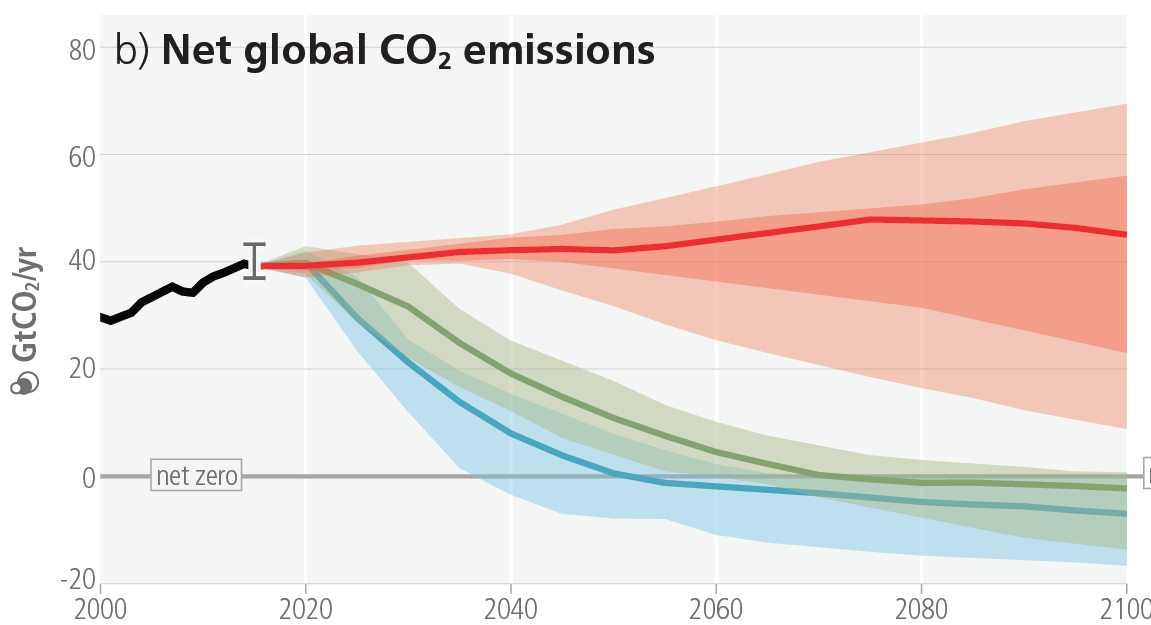
\includegraphics[scale=0.3]{images/CO2IPCC.png}
        \end{center}
    \end{minipage}\hfill
    \begin{minipage}{0.45\textwidth}
        \begin{center}
        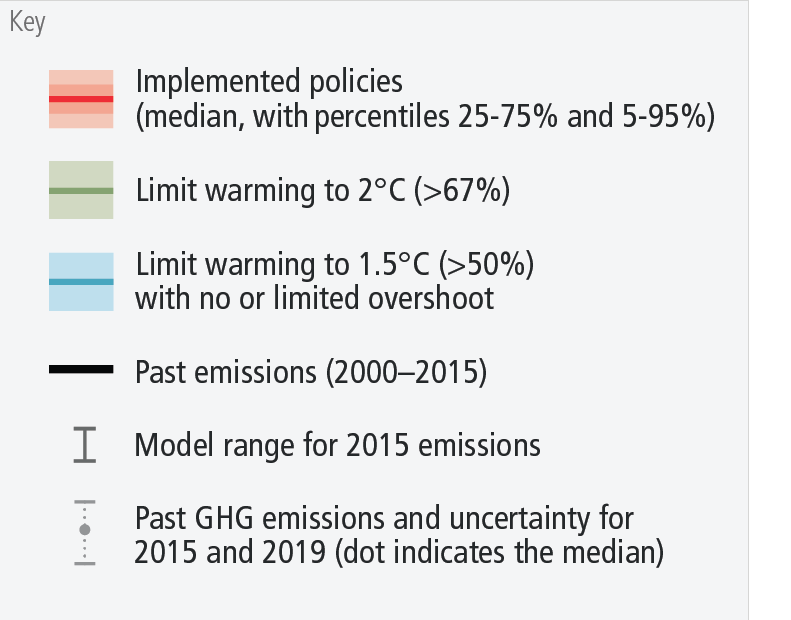
\includegraphics[scale=0.3]{images/legendaIPCC.png}
        \end{center}
    \end{minipage}
    \end{center}
    \caption{CO2 Emissions from the IPCC Report \footnote{IPCC, 2023: Climate Change 2023: Synthesis Report. Available at: \url{https://www.ipcc.ch/report/ar6/syr/}}}
 
\end{figure}

}

\end{frame}
\begin{frame}

\begin{center}
\begin{minipage}{0.7\textwidth}
    \begin{center}
    
\includegraphics[scale=0.5]{images/everythingisfine.jpg}
    \end{center}
\end{minipage}
\end{center}


\end{frame}


\begin{frame}{Energy Grid Transition}

    One of the challenges of transitioning to a fully renewable energy grid comes from two Ducks:
    \\ \bigskip \bigskip
    \pause
    \hspace{3cm}
    
\begin{tikzpicture}
        \duckone
    \end{tikzpicture}
    \hspace{4cm}
    \pause
    
\begin{tikzpicture}
        \ducktwo
    \end{tikzpicture}
   
\end{frame}


\nc{\captionduckone}{\caption{Comparison of Daily Solar Power Generation, Energy Demand, and Net Energy Demand in Italy.\footnote{The Demand, and Solar Power data is taken from the Ninja Dataset at: \url{https://www.renewables.ninja/downloads} }}}
\begin{frame}{Duck one}
\only<1>{
    \begin{figure}[t!]
        \centering
        \begin{tikzpicture}
            %\node  at (axis cs: 3,4) {\duckone};
            \begin{axis}[
                width=15cm,
                height=7cm,
                xlabel={Month},
                ylabel={ \% of energy demand},
                xtick={0, 4, 8, 12, 16, 20},
                xticklabels={00:00, 4:00, 8:00, 12:00, 16:00, 20:00},
                legend pos=north west,
                legend style={draw=none},
                grid=major
            ]
            
            \addplot+[
                thick,
                mark=none,
                color=green!20
            ] table [
                x index=0,
                y index=1,
                col sep=space
            ] {plots/yh_solar.csv};
           
    
            \addplot+[
                thick,
                mark=none,
                color=blue
            ] table [
                x index=0,
                y index=1,
                col sep=space
            ] {plots/yh_demand.csv};
            
    
            \addplot+[
                thick,
                mark=none,
                color=red!20
            ] table [
                x index=0,
                y index=1,
                col sep=space
            ] {plots/yh_net.csv};
            \legend{Solar power, Demand, Unmet Demand};

            \end{axis}

            %\node {\duckone};
    \end{tikzpicture}
    \captionduckone
    \end{figure}
    }
\only<2>{
    \begin{figure}[t!]
        \centering
        \begin{tikzpicture}
            %\node  at (axis cs: 3,4) {\duckone};
            \begin{axis}[
                width=15cm,
                height=7cm,
                xlabel={Hour},
                ylabel={ \% of energy demand},
                xtick={0, 4, 8, 12, 16, 20},
                xticklabels={00:00, 4:00, 8:00, 12:00, 16:00, 20:00},
                legend pos=north west,
                legend style={draw=none},
                grid=major
            ]
            
            \addplot+[
                thick,
                mark=none,
                color=green
            ] table [
                x index=0,
                y index=1,
                col sep=space
            ] {plots/yh_solar.csv};
           
    
            \addplot+[
                thick,
                mark=none,
                color=blue!20
            ] table [
                x index=0,
                y index=1,
                col sep=space
            ] {plots/yh_demand.csv};
            
    
            \addplot+[
                thick,
                mark=none,
                color=red!20
            ] table [
                x index=0,
                y index=1,
                col sep=space
            ] {plots/yh_net.csv};
            \legend{Solar power, Demand, Unmet Demand};

            \end{axis}

            %\node {\duckone};
    \end{tikzpicture}
    \captionduckone
    
    \end{figure}}
\only<3>{
    \begin{figure}[t!]
        \centering
        \begin{tikzpicture}
            %\node  at (axis cs: 3,4) {\duckone};
            \begin{axis}[
                width=15cm,
                height=7cm,
                xlabel={Hour},
                ylabel={ \% of energy demand},
                xtick={0, 4, 8, 12, 16, 20},
                xticklabels={00:00, 4:00, 8:00, 12:00, 16:00, 20:00},
                legend pos=north west,
                legend style={draw=none},
                grid=major
            ]
            
            \addplot+[
                thick,
                mark=none,
                color=green!20
            ] table [
                x index=0,
                y index=1,
                col sep=space
            ] {plots/yh_solar.csv};
           
    
            \addplot+[
                thick,
                mark=none,
                color=blue!20
            ] table [
                x index=0,
                y index=1,
                col sep=space
            ] {plots/yh_demand.csv};
            
    
            \addplot+[
                thick,
                mark=none,
                color=red
            ] table [
                x index=0,
                y index=1,
                col sep=space
            ] {plots/yh_net.csv};
            \legend{Solar power, Demand, Unmet Demand};

            \end{axis}

            %\node {\duckone};
    \end{tikzpicture}
    
    \captionduckone
    \end{figure}}
\only<4>{
    \begin{figure}[t!]
        \centering
        \begin{tikzpicture}
            %\node  at (axis cs: 3,4) {\duckone};
            \begin{axis}[
                width=14cm,
                height=7cm,
                xlabel={Month},
                ylabel={ \% of energy demand},
                xtick={0, 4, 8, 12, 16, 20},
                xticklabels={00:00, 4:00, 8:00, 12:00, 16:00, 20:00},
                legend pos=north west,
                legend style={draw=none},
                grid=major
            ]
            
            \addplot+[
                thick,
                mark=none,
                color=green!20
            ] table [
                x index=0,
                y index=1,
                col sep=space
            ] {plots/yh_solar.csv};
           
    
            \addplot+[
                thick,
                mark=none,
                color=blue!20
            ] table [
                x index=0,
                y index=1,
                col sep=space
            ] {plots/yh_demand.csv};
            
    
            \addplot+[
                thick,
                mark=none,
                color=red
            ] table [
                x index=0,
                y index=1,
                col sep=space
            ] {plots/yh_net.csv};
            \legend{Solar power, Demand, Unmet Demand};
            \end{axis}

            %\node {\duckone};
    \end{tikzpicture}
    
\begin{tikzpicture}
        \duckone
    \end{tikzpicture}
    \captionduckone
    \end{figure}
    % \begin{figure}
    %     \centering
    %     \vspace{-10em}
    %     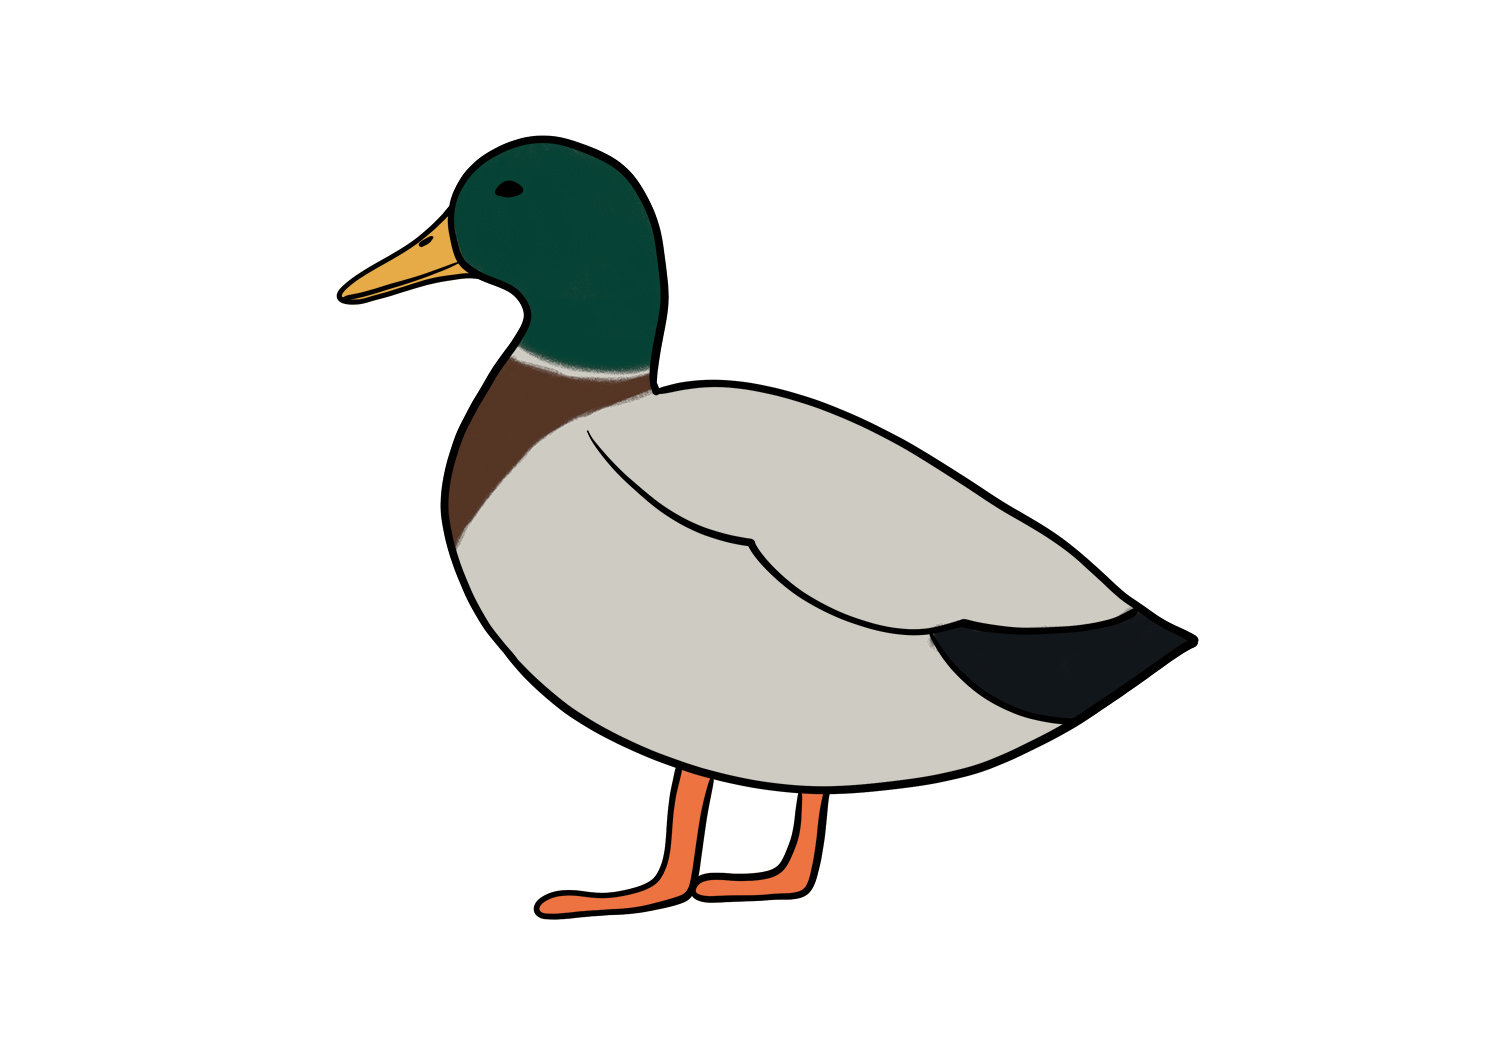
\includegraphics[width=0.5\textwidth]{images/duck.jpg}
    % \end{figure}
    }

    %\includegraphics[width=0.4\textwidth]{duck_joke.png} % Replace with a joke image of a duck
    %\includegraphics[width=0.6\textwidth]{duck_curve.png} % Replace with real duck curve of renewable energy
\end{frame}
\nc{\captionducktwo}{\caption{Comparison of Yearly Solar Power Generation, Energy Demand, and Net Energy Demand in Italy.}}
\begin{frame}{Duck two}
    \only<1>{
\begin{figure}[t!]
    \centering
    \begin{tikzpicture}
        \begin{axis}[
            width=15cm,
            height=7cm,
            xlabel={Month},
            ylabel={ \% of energy demand},
            xtick={0, 63, 120, 180, 240, 310},
            xticklabels={Jan,  Mar,  Jul,  Set, Nov, Dec},
            legend pos=north west,
            legend style={draw=none},
            grid=major
        ]
        
        \addplot+[
            thick,
            mark=none,
            color=green!90
        ] table [
            x index=0,
            y index=1,
            col sep=space
        ] {plots/y3_solar.csv};
       

        \addplot+[
            thick,
            mark=none,
            color=blue!90
        ] table [
            x index=0,
            y index=1,
            col sep=space
        ] {plots/y2_demand.csv};
        

        \addplot+[
            thick,
            mark=none,
            color=red
        ] table [
            x index=0,
            y index=1,
            col sep=space
        ] {plots/y2_net.csv};
        \legend{Solar power, Demand, Net energy}
        \end{axis}
        
        \end{tikzpicture}
        \captionducktwo
\end{figure}
}
\only<2>{
    \begin{figure}[t!]
            \centering
            \begin{tikzpicture}
                %\node  at (axis cs: 3,4) {\duckone};
                \begin{axis}[
                    width=15cm,
                    height=7cm,
                    xlabel={Month},
                    ylabel={ \% of energy demand},
                    xtick={0, 63, 120, 180, 240, 310},
                    xticklabels={Jan,  Mar,  Jul,  Set, Nov, Dec},
                    legend pos=north west,
                    legend style={draw=none},
                    grid=major
                ]
                
                \addplot+[
                    thick,
                    mark=none,
                    color=green!20
                ] table [
                    x index=0,
                    y index=1,
                    col sep=space
                ] {plots/y3_solar.csv};
               
        
                \addplot+[
                    thick,
                    mark=none,
                    color=blue!20
                ] table [
                    x index=0,
                    y index=1,
                    col sep=space
                ] {plots/y2_demand.csv};
                
        
                \addplot+[
                    thick,
                    mark=none,
                    color=red
                ] table [
                    x index=0,
                    y index=1,
                    col sep=space
                ] {plots/y2_net.csv};
                \legend{Solar power, Demand, Unmet Demand};

                \end{axis}
                %\node {\duckone};
        \end{tikzpicture}   
        
\begin{tikzpicture}
            \ducktwo
        \end{tikzpicture}
        \captionducktwo
    \end{figure}}
    

%\includegraphics[width=0.4\textwidth]{duck_joke.png} % Replace with a joke image of a duck
%\includegraphics[width=0.6\textwidth]{duck_curve.png} % Replace with real duck curve of renewable energy

\end{frame}


% \begin{frame}{Energy Storage Planning}
%     %We want to understand where to buiold storage units and renewables
%     %maybe model
%     We consider a two stage stochastic program consisting of a Capacity Expansion Problem (CEP) and an Economic Dispatch (ED) problem:
%     \begin{align*}
%       \min_{x} \quad & c'x + \bE_{\omega}\left[\cV(x,\omega)\right] \\ 
%       s.t. \;   \quad  & 0 \leq x \leq x^{max}
%     \end{align*}
%     Where the Economic dispatch cost is:
%     \begin{align*}
%         \cV(x,\omega) = & \frac{1}{J} \sum_{s \in \cJ} \sum_{t \in \cT} \Bigg(\sum_{i \in \netN}
%     \left( c_i^\aHtE \HtEi + c_i^\aEtH \EtHi \right) + \\
%      & \hspace{2cm} \sum_{l \in \netE_H} \cHedge |\Hedgej| + \sum_{l\in \netE_P} \cPedge |\Pedgej| \Bigg),
%     \end{align*}
%     % \begin{itemize}
%     %     \item The first stage determines the optimal capacities \(x\) for each component of the power grid. %generator \(g \in \cG \) and network component.
%     %     \item The second stage solves the Economic Dispatch for a given time horizon in function of the capacities \(x\) and the scenario \(\omega\), yielding \(\cV(x,\omega)\) as solution.
%     %     % \item Energy Storage Units Expansion need to account both for intra-day variability and yearlong variability
%     %     % \item Model must include many time steps for large time periods,
%     %     % \item over multiple scenarios.
%     %     % \item In general this gives too large models to solve (even if just LPs)
%     % \end{itemize}
% \end{frame}

\section{Why We Need Time Series Aggregation}

\begin{frame}[t]{Capacity Expansion Problem}
    \vspace{0pt}
    \only<1-5>{
    \begin{align*}
             \only<1-5>{ \min_{\xvar} \quad & c'\xvar} \only<2-5>{ + \bE_{\omega}\left[\cV(\xvar,\omega)\right]} \\ 
             \only<3-5>{ s.t. \;   \quad  & 0 \leq \xvar \leq x^{max}}
    \end{align*}
    }
    \only<4-5>{
    Where, given the set of timesteps in the time horizon  \(\cT=\{1,2,\ldots,\Tmax\}\):}
    \only<5-5>{
    \begin{align*}
        \cV(\xvar,\omega) = \min_{\textcolor{black}{\zvar} \in \textcolor{black}{\Zvar}}\sum_{t \in \cT} \Bigg(\sum_{i \in \netN}
    \left( c_i^\aHtE \textcolor{black}{\HtEi} + c_i^\aEtH \textcolor{black}{\EtHi} \right) + \sum_{l \in \netE_H} \cHedge |\textcolor{black}{\Hedgej}| + \sum_{l\in \netE_P} \cPedge |\textcolor{black}{\Pedgej}| \Bigg),
    \end{align*}}
    
    \only<6-10>{
        
        \begin{align*}
             \min_{\xvar} \quad & c'\xvar  + \bE_{\omega}\left[\cV(\xvar,\omega)\right] \\ 
             s.t. \;   \quad  & 0 \leq \xvar \leq x^{max}
        \end{align*}
        
        Where, given the set of timesteps in the time horizon \(\cT=\{1,2,\ldots,\Tmax\}\):
        
        \begin{align*}
            \cV(\xvar,\omega) = \min_{\zvar \in \Zvar}\sum_{t \in \cT} \Bigg(\sum_{i \in \netN}
        \left( c_i^\aHtE \HtEi + c_i^\aEtH \EtHi \right) + \sum_{l \in \netE_H} \cHedge |\Hedgej| + \sum_{l\in \netE_P} \cPedge |\Pedgej| \Bigg),
        \end{align*}
   
   \(\xvar\) rapresents variables corresponding to the componenents expansion in the grid:\\} 
    \only<7-10>{\hspace{1cm}\(\nsi,\;\nwi\;\nhi\):  \myemph{wind turbines}, \myemph{photovotaic panels} and \myemph{hydrogen storage} capacity expansion\\}
    \only<8-10>{\hspace{1cm}\(\addNTCj\), \(\addMHj\): \myemph{transmittion line} and  \myemph{hydrogen pypes} maximum capacity  \\} 
    \only<9-10>{\hspace{1cm}\(\methi,\;\mhtei\): \myemph{electrolyzers and power} cells capacity \\}
    \only<10-10>{\hspace{1cm}\(\nhi\):  \myemph{hydrogen storage} capacity.\\}
    \only<11-14>{ 
            \begin{align*}
                 \min_{\xvar} \quad & c'\xvar  + \bE_{\omega}\left[\cV(\xvar,\omega)\right] \\ 
                 s.t. \;   \quad  & 0 \leq \xvar \leq x^{max}
            \end{align*}
            
            Where, given the set of timesteps in the time horizon \(\cT\):
            
            \begin{align*}
                \cV(\xvar,\omega) = \min_{\zvar \in \Zvar}\sum_{t \in \cT} \Bigg(\sum_{i \in \netN}
            \left( c_i^\aHtE \HtEi + c_i^\aEtH \EtHi \right) + \sum_{l \in \netE_H} \cHedge |\Hedgej| + \sum_{l\in \netE_P} \cPedge |\Pedgej| \Bigg),
            \end{align*}    
    
    \(\zvar\) rapresents variables corresponding to the componenents expansion in the grid:\\\vspace{0.5em}}
    \only<12-14>{\hspace{1cm}\(\HtEi, \EtHi\): conversion from hydrogen to electricity and viceversa.\\\vspace{0.5em}}% at node \(i \in \cN\) at time step \(t \in \cT\) for scenario \(\omega \in \cS\).
    \only<13-14>{\hspace{1cm}\(\Hedgej, \Pedgej\):  flow of hydrogen and power through lines.\\\vspace{0.5em}} 
    \only<14>{\hspace{1cm}\(\HSj\): stored hydrogen capacity}
    \only<15>{
        \begin{align*}
            \min_{\xvar} \quad & c'\xvar  + \bE_{\omega}\left[\cV(\xvar,\omega)\right] \\ 
            s.t. \;   \quad  & 0 \leq \xvar \leq x^{max}
       \end{align*}
       
       Where, given the set of timesteps in the time horizon  \(\cT=\{1,2,\ldots,\Tmax\}\):
       
       \begin{align*}
           \cV(\xvar,\omega) = \min_{\zvar \in \Zvar}\sum_{t \in \cT} \Bigg(\sum_{i \in \netN}
       \left( c_i^\aHtE \HtEi + c_i^\aEtH \EtHi \right) + \sum_{l \in \netE_H} \cHedge |\Hedgej| + \sum_{l\in \netE_P} \cPedge |\Pedgej| \Bigg),
       \end{align*}    
   
    \vspace{1cm}\(\Zvar\): is the set of feasible soluzions to the Economic Dispatch problem: satisying power and hydrogen flow conservation constraints at each node, and magnitude constraints.}
 

\end{frame}
% \begin{frame}{Energy Grid Planning}
%     Sarebbe carino disegnio (o videino) con grafo e animazione mega sbatti della rete in cui succedono cose.
% \end{frame}
\begin{frame}{Challenges of Energy Grid Planning}
    \begin{itemize}
        \uncover<1->{\item Stocasticity requires high number of scenarios.\\}
        \uncover<2->{\item Daily Duck requires high time resolution (minutes/hours)\\}
        \uncover<3->{\item Yearly Duck requires long Time Horizon (years).\\}
        \uncover<4->{\item This makes the problem very large to solve \\}
        \uncover<5->{\item and it cannot be easily simplified by making timesteps longer or with a shorter Time Horizon.}
        \uncover<6->{\item Objective: Having as few time steps as possible, while capturing intra-day and seasonal variability}
        
    \end{itemize}
\end{frame}





\begin{frame}{Time Series Aggregation} 
    % -- FIRST PLOT -- %
    \only<1>{
        \begin{figure}[t!]
            \centering
    
            \begin{tikzpicture}
                \def\xOne{10}
                \def\xTwo{20}
                \def\xThree{30}
                \def\xFour{40}
                \def\xFive{50}
                \def\xSix{60} % <-- Add this line
                \def\xSeven{70}
                \def\xEight{80}
                \def\xNine{90}
                \def\xTen{100}
                \def\xEleven{110}
                \def\xTwelve{120}
    
                \begin{axis}[
                    width=15cm,
                    height=7cm,
                    xlabel={Month},
                    ylabel={\% of energy demand},
                    xtick={0, 63, 120, 180, 240, 310},
                    xticklabels={Jan, Mar, Jul, Sep, Nov, Dec},
                    legend pos=north west,
                    legend style={draw=none},
                    grid=major
                ]
    
                % Original curve
                \addplot+[
                    name path=curve,
                    thick,
                    mark=none,
                    color=blue
                ] table [
                    x index=0,
                    y index=1,
                    col sep=space
                ] {plots/y2_demand.csv};
    
                % Path along x-axis
                \path[name path=baseline] (axis cs:0,0) -- (axis cs:340,0);
    
                % \foreach \start/\color in {
                %     \xOne/blue!20,
                %     \xTwo/green!20,
                %     \xThree/yellow!20,
                %     \xFour/purple!20,
                %     \xFive/red!20,    % 50 to 60
                %     \xSix/cyan!20,  % 60 to 70
                %     \xSeven/orange!20,
                %     \xEight/teal!20,
                %     \xNine/pink!20,
                %     \xTen/lime!20,
                %     \xEleven/brown!20
                % } 
                % \addplot [\color] fill between[
                %     of=curve and baseline, 
                %     soft clip={(\start,-1) rectangle (\start+10,2)}
                % ];
    
                % Shaded regions below the curve with fixed domains
    
            
    
                \legend{Energy Demand};
    
                \end{axis}
            \end{tikzpicture}
            \caption{Energy Demand over a year.}
        \end{figure}
        }
    \only<2>{
    \begin{figure}[t!]
        \centering

        \begin{tikzpicture}
            \def\xOne{10}
            \def\xTwo{20}
            \def\xThree{30}
            \def\xFour{40}
            \def\xFive{50}
            \def\xSix{60} % <-- Add this line
            \def\xSeven{70}
            \def\xEight{80}
            \def\xNine{90}
            \def\xTen{100}
            \def\xEleven{110}
            \def\xTwelve{120}

            \begin{axis}[
                width=15cm,
                height=7cm,
                xlabel={Month},
                ylabel={\% of energy demand},
                xtick={0, 63, 120, 180, 240, 310},
                xticklabels={Jan, Mar, Jul, Sep, Nov, Dec},
                legend pos=north west,
                legend style={draw=none},
                grid=major
            ]

            % Original curve
            \addplot+[
                name path=curve,
                thick,
                mark=none,
                color=blue
            ] table [
                x index=0,
                y index=1,
                col sep=space
            ] {plots/y2_demand.csv};

            % Path along x-axis
            \path[name path=baseline] (axis cs:0,0) -- (axis cs:340,0);

            % \foreach \start/\color in {
            %     \xOne/blue!20,
            %     \xTwo/green!20,
            %     \xThree/yellow!20,
            %     \xFour/purple!20,
            %     \xFive/red!20,    % 50 to 60
            %     \xSix/cyan!20,  % 60 to 70
            %     \xSeven/orange!20,
            %     \xEight/teal!20,
            %     \xNine/pink!20,
            %     \xTen/lime!20,
            %     \xEleven/brown!20
            % } 
            % \addplot [\color] fill between[
            %     of=curve and baseline, 
            %     soft clip={(\start,-1) rectangle (\start+10,2)}
            % ];

            % Shaded regions below the curve with fixed domains

            \addplot [fill=blue!20] fill between[of=curve and baseline, soft clip={(10,0) rectangle (20,2)}];
            \addplot [fill=green!20] fill between[of=curve and baseline, soft clip={(20,0) rectangle (30,2)}];
            \addplot [fill=yellow!20] fill between[of=curve and baseline, soft clip={(30,0) rectangle (40,2)}];
            \addplot [fill=purple!20] fill between[of=curve and baseline, soft clip={(40,0) rectangle (50,2)}];
            \addplot [fill=red!20] fill between[of=curve and baseline, soft clip={(50,0) rectangle (70,2)}];
            \addplot [fill=cyan!20] fill between[of=curve and baseline, soft clip={(70,0) rectangle (80,2)}];
            \addplot [fill=orange!20] fill between[of=curve and baseline, soft clip={(80,0) rectangle (90,2)}];
            \addplot [fill=teal!20] fill between[of=curve and baseline, soft clip={(90,0) rectangle (100,2)}];
            \addplot [fill=pink!20] fill between[of=curve and baseline, soft clip={(100,0) rectangle (110,2)}];
            \addplot [fill=lime!20] fill between[of=curve and baseline, soft clip={(110,0) rectangle (120,2)}];
            \addplot [fill=green!20] fill between[of=curve and baseline, soft clip={(120,0) rectangle (130,2)}];
            \addplot [fill=yellow!20] fill between[of=curve and baseline, soft clip={(130,0) rectangle (140,2)}];
            \addplot [fill=purple!20] fill between[of=curve and baseline, soft clip={(140,0) rectangle (150,2)}];
            \addplot [fill=red!20] fill between[of=curve and baseline, soft clip={(150,0) rectangle (170,2)}];
            \addplot [fill=cyan!20] fill between[of=curve and baseline, soft clip={(170,0) rectangle (180,2)}];
            \addplot [fill=orange!20] fill between[of=curve and baseline, soft clip={(180,0) rectangle (190,2)}];
            \addplot [fill=teal!20] fill between[of=curve and baseline, soft clip={(190,0) rectangle (200,2)}];
            \addplot [fill=pink!20] fill between[of=curve and baseline, soft clip={(200,0) rectangle (210,2)}];
            \addplot [fill=lime!20] fill between[of=curve and baseline, soft clip={(210,0) rectangle (220,2)}];
            \addplot [fill=green!20] fill between[of=curve and baseline, soft clip={(220,0) rectangle (230,2)}];
            \addplot [fill=yellow!20] fill between[of=curve and baseline, soft clip={(230,0) rectangle (240,2)}];
            \addplot [fill=purple!20] fill between[of=curve and baseline, soft clip={(240,0) rectangle (250,2)}];
            \addplot [fill=red!20] fill between[of=curve and baseline, soft clip={(250,0) rectangle (270,2)}];
            \addplot [fill=cyan!20] fill between[of=curve and baseline, soft clip={(270,0) rectangle (280,2)}];
            \addplot [fill=orange!20] fill between[of=curve and baseline, soft clip={(280,0) rectangle (290,2)}];
            \addplot [fill=teal!20] fill between[of=curve and baseline, soft clip={(290,0) rectangle (300,2)}];
            \addplot [fill=pink!20] fill between[of=curve and baseline, soft clip={(300,0) rectangle (310,2)}];
            \addplot [fill=blue!20] fill between[of=curve and baseline, soft clip={(310,0) rectangle (320,2)}];
            \addplot [fill=green!20] fill between[of=curve and baseline, soft clip={(320,0) rectangle (330,2)}];
            \addplot [fill=yellow!20] fill between[of=curve and baseline, soft clip={(330,0) rectangle (340,2)}];
            % \addplot [fill=purple!20] fill between[of=curve and baseline, soft clip={(330,0) rectangle (350,2)}];
            % \addplot [fill=red!20] fill between[of=curve and baseline, soft clip={(350,0) rectangle (370,2)}];
            % \addplot [fill=cyan!20] fill between[of=curve and baseline, soft clip={(370,0) rectangle (380,2)}];
            % \addplot [fill=orange!20] fill between[of=curve and baseline, soft clip={(380,0) rectangle (390,2)}];
            % \addplot [fill=teal!20] fill between[of=curve and baseline, soft clip={(390,0) rectangle (400,2)}];

        
        

            \legend{Energy Demand};

            \end{axis}
        \end{tikzpicture}
        \caption{Energy Demand over a year with highlighted periods.}
    \end{figure}
    }
    \only<4->{
        \begin{figure}[t!]
            \centering
    
            \begin{tikzpicture}
                \def\xOne{10}
                \def\xTwo{20}
                \def\xThree{30}
                \def\xFour{40}
                \def\xFive{50}
                \def\xSix{60} % <-- Add this line
                \def\xSeven{70}
                \def\xEight{80}
                \def\xNine{90}
                \def\xTen{100}
                \def\xEleven{110}
                \def\xTwelve{120}
    
                \begin{axis}[
                    width=15cm,
                    height=7cm,
                    xlabel={Month},
                    ylabel={\% of energy demand},
                    xtick={0, 63, 120, 180, 240, 310},
                    xticklabels={Jan, Mar, Jul, Sep, Nov, Dec},
                    legend pos=north west,
                    legend style={draw=none},
                    grid=major
                ]
    
                % Original curve
                \addplot+[
                    name path=curve,
                    thick,
                    mark=none,
                    color=blue
                ] table [
                    x index=0,
                    y index=1,
                    col sep=space
                ] {plots/y2_demand.csv};
    
                % Path along x-axis
                \path[name path=baseline] (axis cs:0,0) -- (axis cs:350,0);
    
                % \foreach \start/\color in {
                %     \xOne/blue!20,
                %     \xTwo/green!20,
                %     \xThree/yellow!20,
                %     \xFour/purple!20,
                %     \xFive/red!20,    % 50 to 60
                %     \xSix/cyan!20,  % 60 to 70
                %     \xSeven/orange!20,
                %     \xEight/teal!20,
                %     \xNine/pink!20,
                %     \xTen/lime!20,
                %     \xEleven/brown!20
                % } 
                % \addplot [\color] fill between[
                %     of=curve and baseline, 
                %     soft clip={(\start,-1) rectangle (\start+10,2)}
                % ];
    
                % Shaded regions below the curve with fixed domains
    
                \addplot [fill=blue!20] fill between[of=curve and baseline, soft clip={(10,0) rectangle (30,2)}];
                \addplot [fill=green!20] fill between[of=curve and baseline, soft clip={(30,0) rectangle (50,2)}];
                \addplot [fill=yellow!20] fill between[of=curve and baseline, soft clip={(50,0) rectangle (70,2)}];
                \addplot [fill=purple!20] fill between[of=curve and baseline, soft clip={(70,0) rectangle (90,2)}];
                \addplot [fill=red!20] fill between[of=curve and baseline, soft clip={(90,0) rectangle (110,2)}];
                \addplot [fill=cyan!20] fill between[of=curve and baseline, soft clip={(110,0) rectangle (130,2)}];
                \addplot [fill=orange!20] fill between[of=curve and baseline, soft clip={(130,0) rectangle (150,2)}];
                \addplot [fill=teal!20] fill between[of=curve and baseline, soft clip={(150,0) rectangle (170,2)}];
                \addplot [fill=pink!20] fill between[of=curve and baseline, soft clip={(170,0) rectangle (190,2)}];
                \addplot [fill=lime!20] fill between[of=curve and baseline, soft clip={(190,0) rectangle (210,2)}];
                \addplot [fill=green!20] fill between[of=curve and baseline, soft clip={(210,0) rectangle (230,2)}];
                \addplot [fill=yellow!20] fill between[of=curve and baseline, soft clip={(230,0) rectangle (250,2)}];
                \addplot [fill=purple!20] fill between[of=curve and baseline, soft clip={(250,0) rectangle (270,2)}];
                \addplot [fill=red!20] fill between[of=curve and baseline, soft clip={(270,0) rectangle (290,2)}];
                \addplot [fill=cyan!20] fill between[of=curve and baseline, soft clip={(290,0) rectangle (310,2)}];
                \addplot [fill=orange!20] fill between[of=curve and baseline, soft clip={(310,0) rectangle (330,2)}];
                \addplot [fill=teal!20] fill between[of=curve and baseline, soft clip={(330,0) rectangle (350,2)}];
               
            
    
                \legend{Energy Demand};
    
                \end{axis}
            \end{tikzpicture}
            \caption{Energy Demand over a year with highlighted periods.}
        \end{figure}
        }
        \only<3>{
        \begin{figure}[t!]
            \centering
    
            \begin{tikzpicture}
                \def\xOne{10}
                \def\xTwo{20}
                \def\xThree{30}
                \def\xFour{40}
                \def\xFive{50}
                \def\xSix{60} % <-- Add this line
                \def\xSeven{70}
                \def\xEight{80}
                \def\xNine{90}
                \def\xTen{100}
                \def\xEleven{110}
                \def\xTwelve{120}
    
                \begin{axis}[
                    width=15cm,
                    height=7cm,
                    xlabel={Month},
                    ylabel={\% of energy demand},
                    xtick={0, 63, 120, 180, 240, 310},
                    xticklabels={Jan, Mar, Jul, Sep, Nov, Dec},
                    legend pos=north west,
                    legend style={draw=none},
                    grid=major
                ]
    
                % Original curve
                \addplot+[
                    name path=curve,
                    thick,
                    mark=none,
                    color=blue
                ] table [
                    x index=0,
                    y index=1,
                    col sep=space
                ] {plots/y2_demand.csv};
    
                % Path along x-axis
                \path[name path=baseline] (axis cs:0,0) -- (axis cs:350,0);
    
                % \foreach \start/\color in {
                %     \xOne/blue!20,
                %     \xTwo/green!20,
                %     \xThree/yellow!20,
                %     \xFour/purple!20,
                %     \xFive/red!20,    % 50 to 60
                %     \xSix/cyan!20,  % 60 to 70
                %     \xSeven/orange!20,
                %     \xEight/teal!20,
                %     \xNine/pink!20,
                %     \xTen/lime!20,
                %     \xEleven/brown!20
                % } 
                % \addplot [\color] fill between[
                %     of=curve and baseline, 
                %     soft clip={(\start,-1) rectangle (\start+10,2)}
                % ];
    
                % Shaded regions below the curve with fixed domains
    
                \addplot [fill=blue!20] fill between[of=curve and baseline, soft clip={(10,0) rectangle (350,2)}];
             
    
                \legend{Energy Demand};
    
                \end{axis}
            \end{tikzpicture}
            \caption{Energy Demand over a year with highlighted periods.}
        \end{figure}
        }

\end{frame}



\begin{frame}{Time Series Aggregation}
    \begin{columns}
        \column{0.45\textwidth} % First column
        \vspace{2cm} \hfill \\
        \uncover<1->{
            Selecting the length of the time steps corresponds to picking a partition \( \cP \) of the original time horizon \( \cT \): \\
        }
        \vspace{2.5cm}
        \uncover<2->{
            For each time partition \( \cP \) we can define the corresponding Capacity Expansion Problem \( \text{CEP} \). For example if \(\{1,2\}\in \cP\): 
            \\ \vspace{1cm}
            %, where the demand (resp. generation) at each interval corresponds to the sum demand over each timestep in the interval (that is, the area under the graph for each interval).
        }
        
        \column{0.45\textwidth} % Second column
        \uncover<1->{
            \begin{align*}
                \cT &= \{1,2,3,\dots,\Tmax\} \\
                &\Big\downarrow \text{ aggregate time horizon} \\
                \cP &= \Bigl\{\{1,\dots,t_{1}\},\dots,\{t_{k-1},\dots,\Tmax\}\Bigr\}
                \end{align*}
                
                


        \vspace{1cm}}
        
        \uncover<2->{
            \begin{align*}
                &\mCEPT & \xrightarrow{\text{aggregation}} \mCEPP \\
                &\EtHii{1}{}{}, \EtHii{2}{}{} & \xrightarrow{\textcolor{white}{\text{aggregation}}} \EtHii{\{1,2\}}{}{}
              \end{align*}
              
        }

    \end{columns}
\end{frame}

\begin{frame}{Questions}
    1) In what relationships are the Capacity Expansion Problems of different partitions? \\ \vspace{1cm}
    2) When can we obtain a solution of \CEPT given a solution of the aggregated problem \CEPP? \\ \vspace{1cm}
    3) Can we effectively iterate over finer time partitions to obtain a solution of \CEPT?
\end{frame}

\begin{frame}{Row and Column aggregation of CEP}

    % Consider the Capacity Expansion problem for a single scenario of a fully renewable electrical grid as defined in Section \ref{section: model}.
    % %
    % The network is represented by a directed graph \(\cG = (\netN, \netE)\), where \(\netN\) corresponds to the nodes (buses) in the network, and \(\netE = \netE_H \cup \netE_P\) represents transmission lines (\(e \in \netE_P\)) and hydrogen lines (\(e \in \netE_H\)).
    % %
    % At each node \(i\) in the network, \(\nsi\) solar panels and \(\nwi\) wind turbines are installed, where \(\nsi\) and \(\nwi\) are decision variables of the problem. 
    % %
    % At each time-step \(t \in \cT\), each solar panel and wind turbine produces \(\ES\, \power\) and \(\EW \, \power\) respectively. 
    % %
    % Furthermore, at every node \(n\), we have power cells allowing for conversion between electricity and hydrogen, modeled through the variables \(\EtHi\) and \(\HtEi\). 
    % %
    % The power flow through line \(l \in \netE\) is denoted by the variable \(\Pedgej\). 
    % %
    % At each time-step \(t\) and at each node \(i \in \netN\), the power injected into node \(i\) must equal the power demand \(\EL_{i,s,t}\), resulting in the power balance constraint: 
    % \[
    % \ES_{i,s,t}\ns + \EW_{i,s,t}\nwi - \EtHi + \HtEi + \sum_{l \in \inn(i)} \Pedgej - \sum_{l \in \outn(i)} \Pedgej = \EL_{i,s,t}
    % \]
    % %
    % Let us examine the Power Balance constraints \eqref{constr_P} \(r_1\) and \(r_2\) at a fixed node \(i \in\cN\) and time-steps \(t_1\) and \(t_2\), respectively.
    % %
    % We also define the Power Balance constraint \(R\) over the whole time interval \(I = \{t_1,t_2\}\): the power produced by each generator equals the sum of power produced during \(t_1\) and \(t_2\), analogously the same is done for the load. 
    % %
    % For simplicity, we assume that \(i\) is connected to a single other node, and we drop index \(i\) from the variables.
    % %
    % We observe that substituting the constraints \(r_1\) and \(r_2\) with the constraint \(R\) is a structure-preserving aggregation with respect to the function \(f\), as depicted in Figure \ref{ex: spa}, since all the aggregated variables are mapped to variables with the same coefficients.
    % %
    % The same can be done for all other constraints appearing in \CEPT, except for the Hydrogen Storage constraint \eqref{constr_H_storage}, for time-steps \(\bar{t}\) where \(\bar{t}\) is not an extreme of one of the intervals in \(\timeP\), we refer to these constraints as \emph{intermediate Hydrogen Storage Constraints}.
    % %
    % Thus, \CEPP\; is a structure-preserving aggregation of \CEPT\; without the intermediate Hydrogen Storage Constraints.

    \only<1-11>{
    \begin{figure}
    \label{ex: spa}
    \centering
    \begin{tikzpicture}
      [place/.style={circle,thick},
      transition/.style={rectangle,draw=black!50,fill=black!20,thick}]
    
    % Nodes for the first two time-steps
    \uncover<1-11>{
    \node (t1) at (0, 2) {$\ESt{t_1}\ns + \EWt{t_1}\nw - \EtHii{t_1}{}{} + \HtEii{t_1}{}{} + \Pedgejj{j}{t_1}{} = \ELt{t_1}$};
    \node[circle, minimum size=0.6cm] (nst1) at (-3.1, 2) {};
    \node[circle, minimum size=0.6cm] (nwt1) at (-1.2, 2) {};
    \node[circle, minimum size=0.6cm] (EtHt1) at (-0.1,  2) {};
    \node[circle, minimum size=0.6cm] (HtEt1) at (1.1,  2) {};
    \node[circle, minimum size=0.6cm] (Pt1) at (2.2,  2) {};
    }
    
    \uncover<2-11>{
    \node (t2) at (0, 0) {$\ESt{t_2}\ns + \EWt{t_2}\nw - \EtHii{t_2}{}{} + \HtEii{t_2}{}{} + \Pedgejj{l}{t_2}{} = \ELt{t_2}$};
    \node[circle, minimum size=0.6cm] (nst2) at (-3.5, 0) {};
    \node[circle, minimum size=0.6cm] (nwt2) at (-1.4, 0) {};
    \node[circle, minimum size=0.6cm] (EtHt2) at (-0.1,  0) {}; 
    \node[circle, minimum size=0.6cm] (HtEt2) at (1.7,  0) {};
    \node[circle, minimum size=0.4cm] (Pt2) at (2.4,  0) {};
    }

    % Node for the aggregated constraint
    \uncover<3-11>{
    \node (T) at (0, -2) {$(\ESt{t_1} + \ESt{t_2})\ns + (\EWt{t_1} + \EWt{t_2})\nw - \EtHii{\{t_1,t_2\}}{}{} + \HtEii{\{t_1,t_2\}}{}{} + \Pedgejj{l}{\{t_1,t_2\}}{} = \ELt{\{t_1,t_2\}}$};
    \node[circle, minimum size=0.7cm] (nstT) at (-3.8, -2) {};
    \node[circle, minimum size=0.6cm] (nwtT) at (-0.4, -2) {};
    \node[circle, minimum size=0.8cm] (EtHtT) at (0.9, -2) {};
    \node[circle, minimum size=0.6cm] (HtEtT) at (2.3, -2) {};
    \node[circle, minimum size=0.6cm] (PtT) at (3.6, -2) {};
    }
    % Arrows from aggregated constraint to time-step 1
    \uncover<4-11>{
    \draw[violet!50!magenta, thick, <-, rounded corners] (nstT) .. controls (-4.5, -1) and (-5, 1)  .. node[right, near end] {$\neq$} (nst1);}
    \uncover<5-11>{
    \draw[violet!50!magenta, thick, <-, rounded corners] (nwtT) .. controls (0.2, -1) and (-2.0, 1)  .. node[right, near end] {$\neq$}(nwt1);}
    \uncover<6-11>{
    \draw[violet, thick, <-, rounded corners] (EtHtT) .. controls (0.6, -1) and (0.6, 1)  .. node[right, near end] {$=$}(EtHt1);}
    \uncover<7-11>{
    \draw[violet, thick, <-, rounded corners] (HtEtT) .. controls (2.2, 0) and (1.6, 1)  .. node[right, near end] {$=$}(HtEt1);}
    \uncover<8-11>{
    \draw[violet, thick, <-, rounded corners] (PtT) .. controls (5, -1) and (4.5, 0.5)  .. node[right, near end] {$=$}(Pt1);}
    
    % Arrows from aggregated constraint to time-step 2
    \uncover<9-11>{
    \draw[blue!50!cyan, thick, <-, rounded corners] (nstT) .. controls (-3.0, -1.5) and (-3.4, -0.5)  .. node[right] {$\neq$}(nst2);}
    \uncover<10-11>{
    \draw[blue!50!cyan, thick, <-, rounded corners] (nwtT) .. controls (-0.4, -1) and (-1.2, -0.5)  .. node[right] {$\neq$} (nwt2);}
    \uncover<10-11>{
    \draw[blue, thick, <-, rounded corners] (EtHtT) .. controls (0.3, -1.5) and (-0.1, -0.5)  .. node[right] {$=$} (EtHt2);}
    \uncover<10-11>{
    \draw[blue, thick, <-, rounded corners] (HtEtT) .. controls (2.2, -1.5) and (1.1, -0.5)  .. node[right] {$=$}(HtEt2);}
    \uncover<10-11>{
    \draw[blue, thick, <-, rounded corners] (PtT) .. controls (3.3, -1.5) and (2.5, -0.5)  .. node[right] {$=$}(Pt2);}
    
    % Legends for f^t1 and f^t2
    \uncover<8-11>{
    \node[below right] at (-6.3, 1.8) {\textcolor{violet}{\large $f|_{\supp(\Av_{r_1})}$}};}
    \uncover<11-11>{
    \node[below right] at (-6.5, -0.5) {\textcolor{blue}{\large $f|_{\supp(\Av_{r_2})}$}};}
    
    \end{tikzpicture}

    \end{figure}
    }
    \only<12>{
        \begin{figure}
        
        \centering
        \begin{tikzpicture}
          [place/.style={circle,thick},
          transition/.style={rectangle,draw=black!50,fill=black!20,thick}]
        
        % Nodes for the first two time-steps
        \node (t1) at (0, 2) {$\ESt{t_1}\ns + \EWt{t_1}\nw - \EtHii{t_1}{}{} + \HtEii{t_1}{}{} + \Pedgejj{j}{t_1}{} = \ELt{t_1}$};
        \node[circle, minimum size=0.6cm] (nst1) at (-3.1, 2) {};
        \node[circle, minimum size=0.6cm] (nwt1) at (-1.2, 2) {};
        \node[circle, minimum size=0.6cm] (EtHt1) at (-0.1,  2) {};
        \node[circle, minimum size=0.6cm] (HtEt1) at (1.1,  2) {};
        \node[circle, minimum size=0.6cm] (Pt1) at (2.2,  2) {};
        
        
        \node (t2) at (0, 0) {$\ESt{t_2}\ns + \EWt{t_2}\nw - \EtHii{t_2}{}{} + \HtEii{t_2}{}{} + \Pedgejj{l}{t_2}{} = \ELt{t_2}$};
        \node[circle, minimum size=0.6cm] (nst2) at (-3.5, 0) {};
        \node[circle, minimum size=0.6cm] (nwt2) at (-1.4, 0) {};
        \node[circle, minimum size=0.6cm] (EtHt2) at (-0.1,  0) {}; 
        \node[circle, minimum size=0.6cm] (HtEt2) at (1.7,  0) {};
        \node[circle, minimum size=0.4cm] (Pt2) at (2.4,  0) {};
        % Node for the aggregated constraint
        \node (T) at (0, -2) {$(\ESt{t_1} + \ESt{t_2})\ns + (\EWt{t_1} + \EWt{t_2})\nw - \EtHii{\{t_1,t_2\}}{}{} + \HtEii{\{t_1,t_2\}}{}{} + \Pedgejj{l}{\{t_1,t_2\}}{} = \ELt{\{t_1,t_2\}}$};
        \node[circle, minimum size=0.7cm] (nstT) at (-3.8, -2) {};
        \node[circle, minimum size=0.6cm] (nwtT) at (-0.4, -2) {};
        \node[circle, minimum size=0.8cm] (EtHtT) at (0.9, -2) {};
        \node[circle, minimum size=0.6cm] (HtEtT) at (2.3, -2) {};
        \node[circle, minimum size=0.6cm] (PtT) at (3.6, -2) {};
        
        % Arrows from aggregated constraint to time-step 1
        \draw[violet!50!magenta, thick, ->, rounded corners] (nstT) .. controls (-4.5, -1) and (-5, 1)  .. node[right, near end] {$\neq$} (nst1);
        
        \draw[violet!50!magenta, thick, ->, rounded corners] (nwtT) .. controls (0.2, -1) and (-2.0, 1)  .. node[right, near end] {$\neq$}(nwt1);
        
        \draw[violet, thick, ->, rounded corners] (EtHtT) .. controls (0.6, -1) and (0.6, 1)  .. node[right, near end] {$=$}(EtHt1);
        
        \draw[violet, thick, ->, rounded corners] (HtEtT) .. controls (2.2, 0) and (1.6, 1)  .. node[right, near end] {$=$}(HtEt1);
        
        \draw[violet, thick, ->, rounded corners] (PtT) .. controls (5, -1) and (4.5, 0.5)  .. node[right, near end] {$=$}(Pt1);
        % Arrows from aggregated constraint to time-step 2
        \draw[blue!50!cyan, thick, ->, rounded corners] (nstT) .. controls (-3.0, -1.5) and (-3.4, -0.5)  .. node[right] {$\neq$}(nst2);
        
        \draw[blue!50!cyan, thick, ->, rounded corners] (nwtT) .. controls (-0.4, -1) and (-1.2, -0.5)  .. node[right] {$\neq$} (nwt2);
        
        \draw[blue, thick, ->, rounded corners] (EtHtT) .. controls (0.3, -1.5) and (-0.1, -0.5)  .. node[right] {$=$} (EtHt2);
        
        \draw[blue, thick, ->, rounded corners] (HtEtT) .. controls (2.2, -1.5) and (1.1, -0.5)  .. node[right] {$=$}(HtEt2);
        
        \draw[blue, thick, ->, rounded corners] (PtT) .. controls (3.3, -1.5) and (2.5, -0.5)  .. node[right] {$=$}(Pt2);
        
        \node[circle] (question) at (-1,1) {\huge{\textcolor{sera}{\textbf{?}}}};
        % Legends for f^t1 and f^t2
    
        
        \end{tikzpicture}
        \end{figure}
        }
    
\end{frame}
\begin{frame} {(1) In what relationships are the Capacity Expansion Problems fo different partitions? }
%    \uncover<1->{
%     Constructing \CEPP  to a rows and columns aggregation of the LP problem associated to \CEP. Where a (or more) subset of rows is substituted with one single row equal to a linear combination of the rows in the subset. And the same is done to the columns of the constraint matrix. \\ \vspace{1cm}}

    \uncover<1->{
        \begin{observation}
            Row aggregations are always relaxations of the original problem. 
        \end{observation}
    }
    \vspace{1.5cm}
    \uncover<2->{
        \begin{observation}
            Column aggregation are relaxations\footnote{Where by relaxation we mean that there is a cost preserving map from the feasible solution set of the original problem and the feasible solution set of the relaxed problem.} if the non-zero rows of the of the aggregated columns are equal. 
        \end{observation}
     
    }
    \vspace{1cm}
    \uncover<3->{
        Thus given a sequence of finer time partitions \(\cP_1 \leq \cP_2 \leq \ldots \leq \cP_n = \cT\) we obtain tighter and tigher relaxations \(\text{\CEP}_{\cP_i}\) whose optimal cost is eventually equal to the optimal cost of \CEPT.
    }
\end{frame}
     
   
\section{Structure-Preserving Aggregations}

\begin{frame}{General definition of Structure Preserving Aggregation}

\begin{definition}
    \label{def:structure preserving aggregation}
    Given an LP, a row and column aggregation with respect to partitions \(\rowP,  \colP\) is said to be \myemph{structure-preserving} if \(f:[n] \rightarrow [\tilde{n}]\)
    %
    \pause, given by
    \[
    f : c \mapsto C \quad \text{ where } C \text{ is the element in } \colP \text{ such that } c\in C,
    \]
    \pause is such that for each \(R \in \rowP_{>1}\) and all \(r \in R\):
    \[
    f|_{\supp(\Av_r)} : \supp(\Av_r) \rightarrow \supp(\At_R)
    \]
    is a bijection, and \pause
    \[
    \Av_{r,c} = \At_{R,f(c)} \quad \text{for all } c \in \supp(\Av_r)_{>1}.
    \]
  \end{definition}
\end{frame}

\begin{frame}{(2) When can we obtains a solution of \CEPT given a solution of the aggregated problem \CEPP? \\ \vspace{1cm}}
    Given a solution \(\xt\) of the aggregated problem \CEPP, we want to extend it to a solution \(\xv\) of \CEPT. \\
    \only<1>{ 
    What is a good candidate solution? We keep unaggregated variables the same, that is:
    \[
        \nhi \coloneqq \nhit,\; \nsi \coloneqq \nsit, \; \nsi \coloneqq \nsit
    \]}
    \uncover<2-5>{
    How do we define unaggregated variables? Remember that:
    \[
    \sum_{t \in \{1,\ldots,t_1\}} \HtEii{t}{}{} = \HtEii{\{1,\ldots,t_1\}}{}{}
    \]}
    \uncover<3-5>{
    So we define for all \(t \in \{t,\ldots,t_1\}\):
    \[
        \HtEii{t}{}{} = \rho_t\HtEii{\{1,\ldots,t_1\}}{}{}
    \]}
    \uncover<4-5>{
    Where \(\rho_t\) corresponds to \(\frac{\text{Net power at time t}}{\text{Total Net power at interval} \{1,\ldots,t_1\}}\).
    }
    \uncover<5>{
        \begin{proposition}
            Is such a solution \(\xv\) of \CEPT is well defined, and \(\rho_t \geq 0\), then it is optimal.
        \end{proposition}
    }
\end{frame}
\begin{frame}{Generalization to structure preserving aggregations}
Given a solution \(\xt\) of the aggregated problem \(\tilde{\text{LP}}\), we want to extend it to a solution \(\xv\) of LP. \\
We keep unaggregated vairiables the same, that is, if \(\{c\} \in \colP\), then \(\xv_c = \xt_c\). \\ 
Otherwise, for a given aggregated variable \(c \in C\) in the support of the row \(r\) we search solution of the form: 
\begin{align}
\xv_c \coloneqq \rhov_r \xt_{f(c)} \; 
\end{align}
Then:
    \begin{align}
        \Av_r \xv &=\Av_{r, \colP_{=1}} \xv_{\colP_{=1}} + \sum_{c \in \supp(\Av_r)_{>1}} \A_{r, c} \xv_{c} = \Av_{r, \colP_{=1}} \xv_{\colP_{=1}} + \sum_{c \in \supp(\Av_r)_{>1}} \At_{R, f(c)} \xv_{c}  \\
         &=  \Av_{r, \colP_{=1}} \xt_{\colP_{=1}} + \rhov_r \sum_{\col \in \supp(\At_R)_{>1}} \At_{R, \col}  \xt_{\col} = b_r
    \end{align}
    Since \(\sum_{\col \in \supp(\At_R)_{>1}} \At_{R, \col}  \xt_{\col} = \bt_r
    - \At_{R, \colP_{=1}} \xt_{\colP_{=1}}\), the equality holds if and only if:
    \begin{align}
        \rhov_r \coloneqq \frac{\bv_r - \Av_{r, \colP_{=1}} \xt_{\colP_{=1}}}{\bt_r
            - \At_{R, \colP_{=1}} \xt_{\colP_{=1}}}.
    \end{align}
\end{frame}

\begin{frame}{Generalization to structure preserving aggregations}
    \begin{proposition}
        \label{ob:aggrconstr}
       Let \(\xt\) be a solution to the aggregated problem, define 
        \[\rhov_r \coloneqq \frac{\bv_r - \Av_{r, \colP_{=1}} \xt_{\colP_{=1}}}{\bt_r
            - \At_{R, \colP_{=1}} \xt_{\colP_{=1}}}.\]
        If \(\rhov_r \geq 0\) and \(\xv \in \bR^n\) satisfies \(\xv_{\colP_{=1}} = \xt_{\colP_{=1}}\) and \(\xv_{c} = \rhov_r \xt_{f(c)}\) for all \(c \in \supp(\Av_r)_{>1}\), then \(\xv\)  satisfies the constraints \(\Av_r \xv = \bv_r\) and \(\xv_{\supp(\Av_r)} \geq 0\) of the original problem.
    \end{proposition}
    
    Whenever such a solution is well defined we refer to it as a \(\rho\)-solution.
\end{frame}
% \begin{frame}{rho solutions}

%     \begin{definition}
%         Let \(\rhov_r\) be defined as in Observation \ref{ob:aggrconstr} for all \(r \in R \in \rowP_{>1}\). Let \(\xv \in \bR^n\) be defined as \(\xv_{\colP_{=1}} \coloneqq \xt_{\colP_{=1}}\) and \(\xv_{c} \coloneqq \rhov_r \xt_{f(c)}\) for all  \(r \in R \in \rowP_{>1}\) and \(c \in \supp(\Av_r)\). 
%         %
%         Then, \(\xv\)  is well defined if and uncover if for all \(r, r' \in R \in \rowP_{>1}\) such that \(\supp(\Av_r) \cap \supp(\Av_{r'})\neq 0\), we have \(\rhov_r = \rhov_{r'}\). 
%         %
%         If \(\rhov \geq 0\), we refer to \(\xv\)  as a \(\rhov\)-solution. 
%       \end{definition}
% \end{frame}


\begin{frame}{(3) Can we effectively iterate over finer time partitions to obtain a solution to \CEPT?}
\begin{enumerate}
    \item Impose the constraints relative to an initial time partition and solve the corresponding LP.
    %
    \item Select a time interval such that either \(\rho_r < 0\) or the \(\rho\)-solution is not well defined and refine it into smaller sub-intervals.
    %
    \item Add the constraints relative to each sub-interval of the selected interval. Solve the model again but using a warm-start.
    %
    \item Repeat steps 2 and 3 until a specified halting condition is met.
    \end{enumerate}
    \vspace{1cm}
    Halting condition:
    \begin{enumerate}
        \item \(\rhov_r\) is constant over the hypergraph associated to the aggregated problem \CEPP and  and \(\rhov \geq 0\). \label{eq: condition 2 iter}
        \item A maximum number of iterations is reached
    \end{enumerate}
    
    \begin{observation}
        If the algorithm alts before the second condition is met, then the \(\rho\)-solution is well defined and is an optimal solution for \CEPT.
    \end{observation}
\end{frame}

\section{Results}

\begin{frame}{Computational Results}
    \begin{itemize}
        \item 5-node network simulation
        \item Comparison of random vs heuristic-based refinement
        \item Faster convergence with structure-preserving methods
    \end{itemize}


\begin{figure}[t!]
    \centering
    \begin{tikzpicture}[scale=0.9]
    \begin{axis}[
        xlabel={Iteration number},
        ylabel={Cost (Millions of Euros)},
        legend pos=north west,
        legend style={draw=none},
        grid=major,
        thick,
        cycle list name=color list,
        yticklabel style={
                /pgf/number format/fixed,        % Use fixed-point notation
                /pgf/number format/precision=4,  % Set precision to 4 decimal places
                /pgf/number format/fixed zerofill % Add trailing zeros if necessary
            }]
    % Importing rho data
    \addplot+[
        thick,
        mark=none,
        color=blue
    ] table[x index=0, y index=1, col sep=space] {plots/costs_rho.csv};
    % Importing random data
    \addplot+[
        thick,
        mark=none,
        color=green
    ] table[x index=0, y index=1, col sep=space] {plots/costs_random.csv};
    % Legend
    \legend{rho, random}
    \end{axis}
    \end{tikzpicture}
    \caption{Cost over iterations of rho selection method versus random selection method}
      \label{fig:rho_vs_average}
\end{figure}
    
\end{frame}

\begin{frame}

    \begin{figure}[t!]
        \centering
        \begin{tikzpicture}[scale=0.9]
        \begin{axis}[
            xlabel={Iteration number},
            ylabel={Total capacity (Kg)},
            legend pos=south east,
            legend style={draw=none},
            grid=major,
            thick,
            cycle list name=color list,
            yticklabel={\pgfmathprintnumber[fixed, precision=5]{\tick}} 
        ]
        
        \addplot+[
            thick,
            mark=none,
            color=blue
        ] table[x index=0, y index=1, col sep=space] {plots/mhte_rho.csv};
        
        \addplot+[
            thick,
            mark=none,
            color=green
        ] table[x index=0, y index=1, col sep=space] {plots/mhte_random.csv};
        
        \legend{rho, random}
        \end{axis}
        \end{tikzpicture}
        \caption{Hydrogen to Power Capacity over iterations}
          \label{fig:mhte_over_iter}
        \end{figure}
        
\end{frame}
\begin{frame}{Conclusion}
    \begin{itemize}
        \item Time series aggregation reduces computational costs
        \item Preserves structure and accuracy
        \item The index \(\rho\) can also be interpreted as a fractional net power production index.
        \item Future direction: Is there always a non trivial time aggregation which induces a tight relaxation of \CEPT?
    \end{itemize}
\end{frame}
\end{document}